\chapter{Seznámení s aplikací}
\label{3-seznameni-s-aplikaci}

\section{Navázání na projekt FGIS}

Tato diplomová práce navazuje na započatý projekt z předmětu Free
%% ML: ja -> autor prace
Software GIS. Na projektu jsem se účastnil já, Tomáš Lauwerys a Michal
Zíma. Projekt měl za úkol vytvořit jednoduchou webovou aplikaci, kdy
%% ML: dat -> zaznamy
přihlášení uživatelé mohli zobrazovat, vytvářet, editovat a mazat dat
z databáze. Databáze pro tento projekt byla pouze cvičná a obsahovala
pouze několik tabulek s textovými poli. Projekt ovšem nebyl zcela
dokončen, protože se nepovedlo vytvořit všechny funkce tak, aby
správně fungovali. Data do databáze šla přidávat, dali se zobrazovat a
také mazat, ale při editaci se po uložení nepřepsala aktuální data v
databázi.

\begin{figure}[H] \centering
    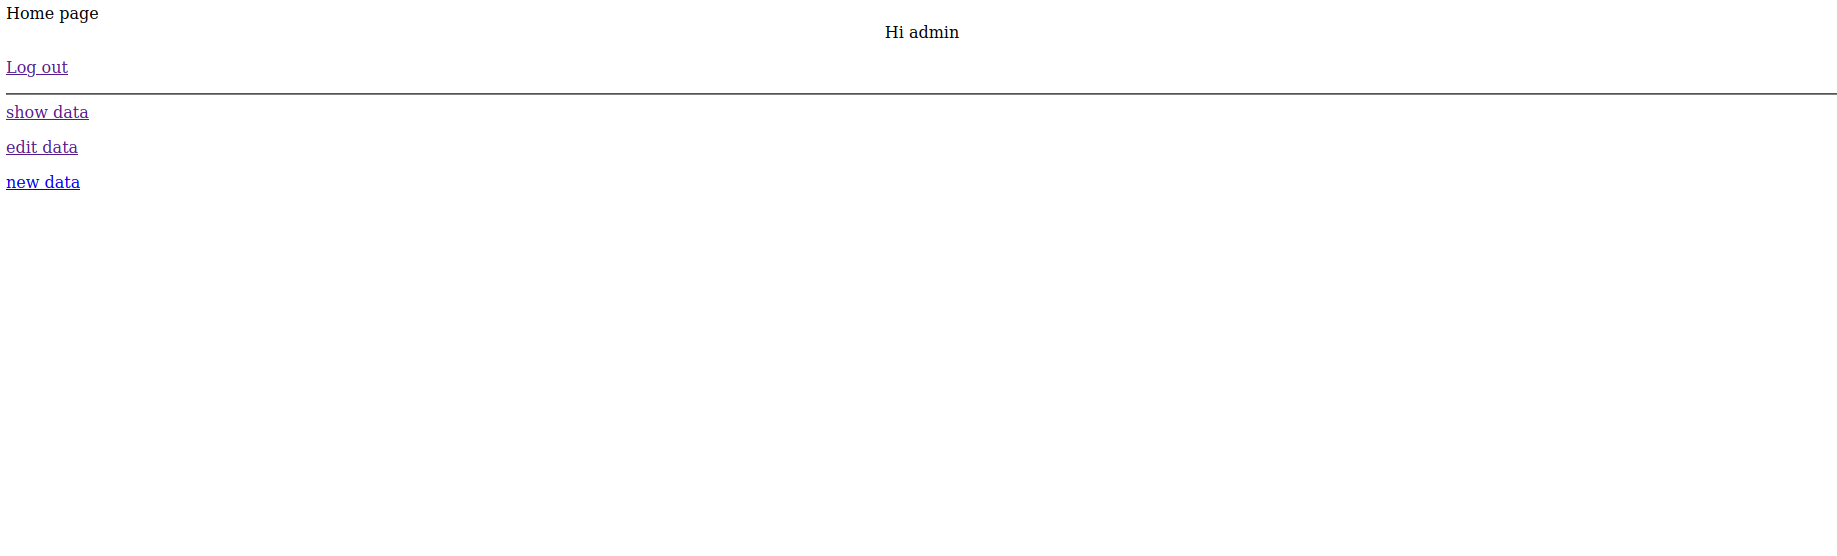
\includegraphics[width=400pt]{./pictures/4-nahled-menu-fgis.PNG}
    \caption[Náhled aplikace vytvořené v projektu FGIS]{Náhled aplikace vytvořené v projektu FGIS}
	\label{fig:Náhled aplikace}              
\end{figure}

 \newpage
 
 \section{O aplikaci}

 V aplikaci jsou použity pohledy založeny na třídách, které se v
 Pythonu používají pro nahrazení pohledů jako funkcí. Použity jsou
 základní pohledy jako ListView pro zobrazení většího obsahu tabulky
 nebo CreateView pro uložení dat do databáze. V aplikaci v soubory
 \emph{views.py} jsou tedy vytvořeny třídy pohledů pro každou URL
 adresu. V souboru \emph{urls.py} jsou propojeny URL adresy, pohledy a
 HTML šablony, na které se odkazují. Složka \emph{templates} poté
 obsahuje html soubory jednotlivých zobrazovaných stránek. Dále je v
 aplikaci v \emph{models.py} zobrazena struktura celé databáze.

 V adresáři projektu je pak v \emph{settings.py} nastaveno připojení k
 databázi, importována django aplikace, připojen adresář obsahující
 složku \emph{templates} nebo nastavení domovské adresy. Soubor
 \emph{urls.py} kromě administrátorské stránky také obsahuje připojení
 aplikace, kde se tedy odkazuje na soubor \emph{urls.py} v adresáři
 aplikace.

\textcolor{red}{přiložit obrázky souborů?}


